% Chapter 1

\section{Hypergraphs} % Main chapter title

\label{Chapter4_hg} % For referencing the chapter elsewhere, use \ref{Chapter1} 
%\label{sec:introduction}
%----------------------------------------------------------------------------------------

%----------------------------------------------------------------------------------------

The Hypergraph, is a generalization of a graph. In contrast to a simple graph, hypergraph's edges can connect multiple vertices. We formally define a hypergraph as $H = (V, E)$ where $V$ is a set of unique {\em vertices} or {\em nodes} and $E$ is the set of {\em edges} or {\em hyperedges}. 
\begin{figure}
	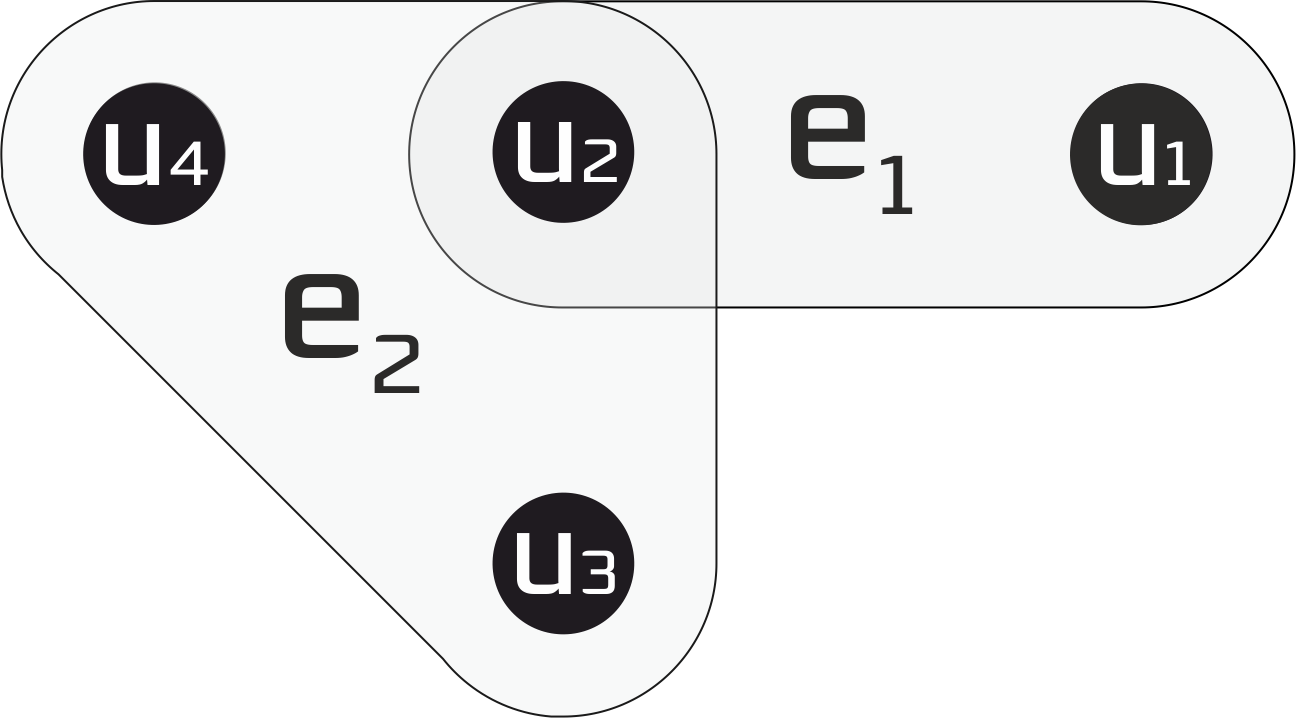
\includegraphics[scale=1]{simple_hg.png}
	\caption{A Simple Hypergraph}
	\label{simplehg}
\end{figure}

A simple hypergraph can be seen in figure~\ref{simplehg}. In this example, the vertices of the hypergraph are $V = \{u_1, u_2, u_3, u_4\}$ and the edges $E = \{e_1, e_2\}$. Edge $e_1$ contains vertices $u_1, u_2$, while $e_2$ contains $u_2, u_3, u_4$.

The difference of graphs and hypergraphs is outlined in the figure of the hyperedge $e_2$~\ref{hyperedge}. As shown, a hyperedge can connect multiple vertices, in contrast to simple graphs where an edge always connects two nodes.

\begin{figure}
	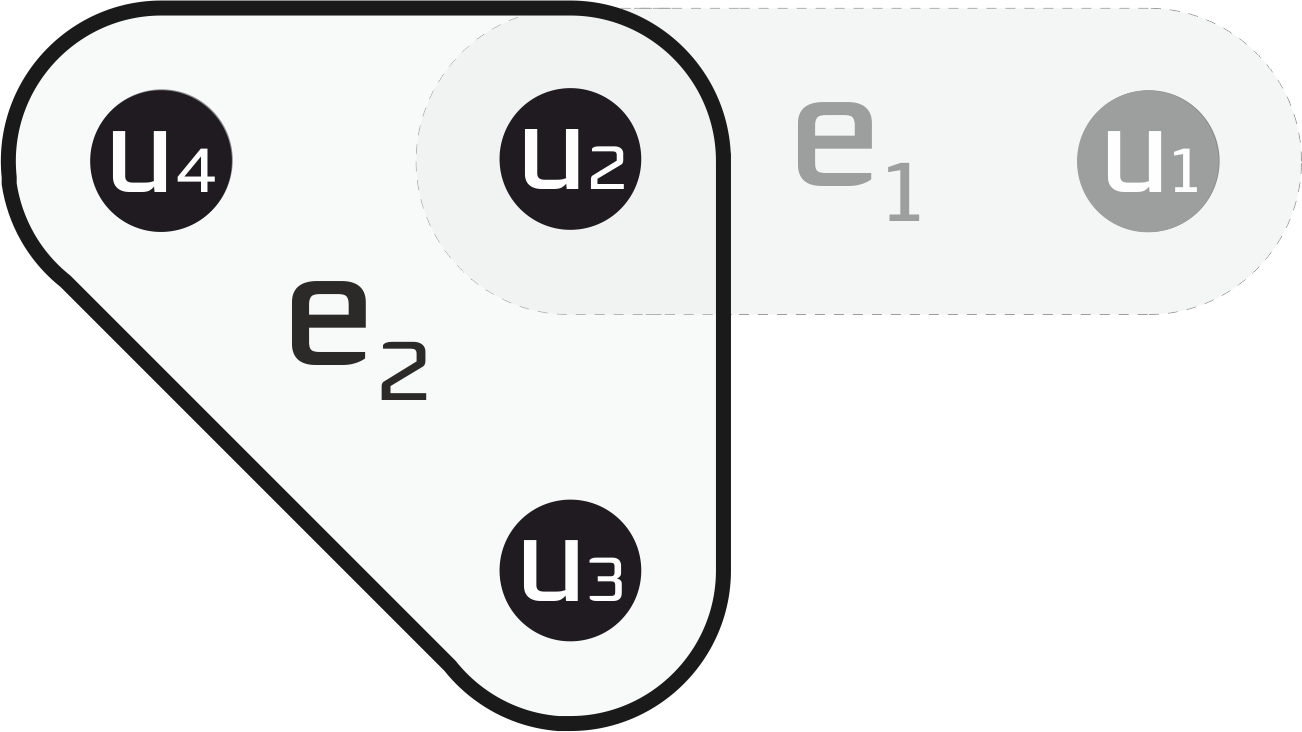
\includegraphics[scale=1]{simple_hyperedge.png}
	\caption{A Single Hyperedge}
	\label{hyperedge}
\end{figure}

Hypergraphs are well studied, and thus there are many definitions in literature which can help us use them as a data structure. First, a {\em transversal}, or {\em hitting set}, of a hypergraph is a set of nodes $T \subset V$ such that T intersects with any edge $E$ of the hypergraph. A {\em hitting set} that does not contain any other hitting set is called {\em minimal}. This is better illustrated in Fig.~\ref{transversalexample}. As shown, the hypergraph has three {\em minimal transversals}: $T_1 = \{u_1, u_4\}, T_2 = \{u_1, u_3\}$ and $T_3 = \{u_2\}$. Any other transversal such as $T_4 = \{u_2, u_4\}$ is not minimal since $T_3 \subset T_4$ (it contains at least one other transversal). Finally, the {\em set of minimal transversals} is called the {\em dual} of a hypergraph or {\em minimal set-cover} and denoted as $H^d$. 

We expect this problem to be of high complexity since it is essentially the set-cover problem extended to hypergraphs. The search version of the set-cover problem in graphs is NP-hard. However, computing the dual hypergrah is a problem widely studied, and hence, many algorithms offer efficient solutions. To begin, Berge's algorithm~\cite{berge1989hypergraphs}, while slower than the rest, is foundation of many algorithms which are merely an improvement on it. Specifically, the algorithms described here, are divided in two types: improvements over Berge and hill-climbing algorithms. The Berge algorithm updates the set of minimal transversals by iteratively adding hyperedges.

Dong and Li~\cite{dong2005mining}, for instance, is a Berge-based algorithm that improves upon it. This method decreases the search space by avoiding to generate several non-minimal transversals. Bailey {\em et al.}~\cite{bailey2003fast} algorithm, starts with a limited vertex set and update both hyperedges and hitting sets by constantly adding new vertices. Kavvadias {\em et al.}
~\cite{kavvadias2005efficient} propose a memory-bound depth-first approach which generates a constant stream of minimal hitting sets. Nevertheless this method does not come with a time complexity bound. Khachiyan {\em et al.}~\cite{boros2003efficient} provide a {\em quasi-polynomial} algorithm for enumerating all minimal transversals. In a sense of time complexity this is the fastest of the algorithms presented here, but in practice it falls behind in several test-cases. Extending on that, another publication~\cite{khachiyan2005new} finds a multi-threaded solution with excellent time complexity assuming multiple cores. Finally~\cite{hebert2007data}, a solution not based on Berge, offers a hill-climbing algorithm that adds vertices in increasing order and checks if they satisfy a minimal transversal condition.
\begin{figure}
	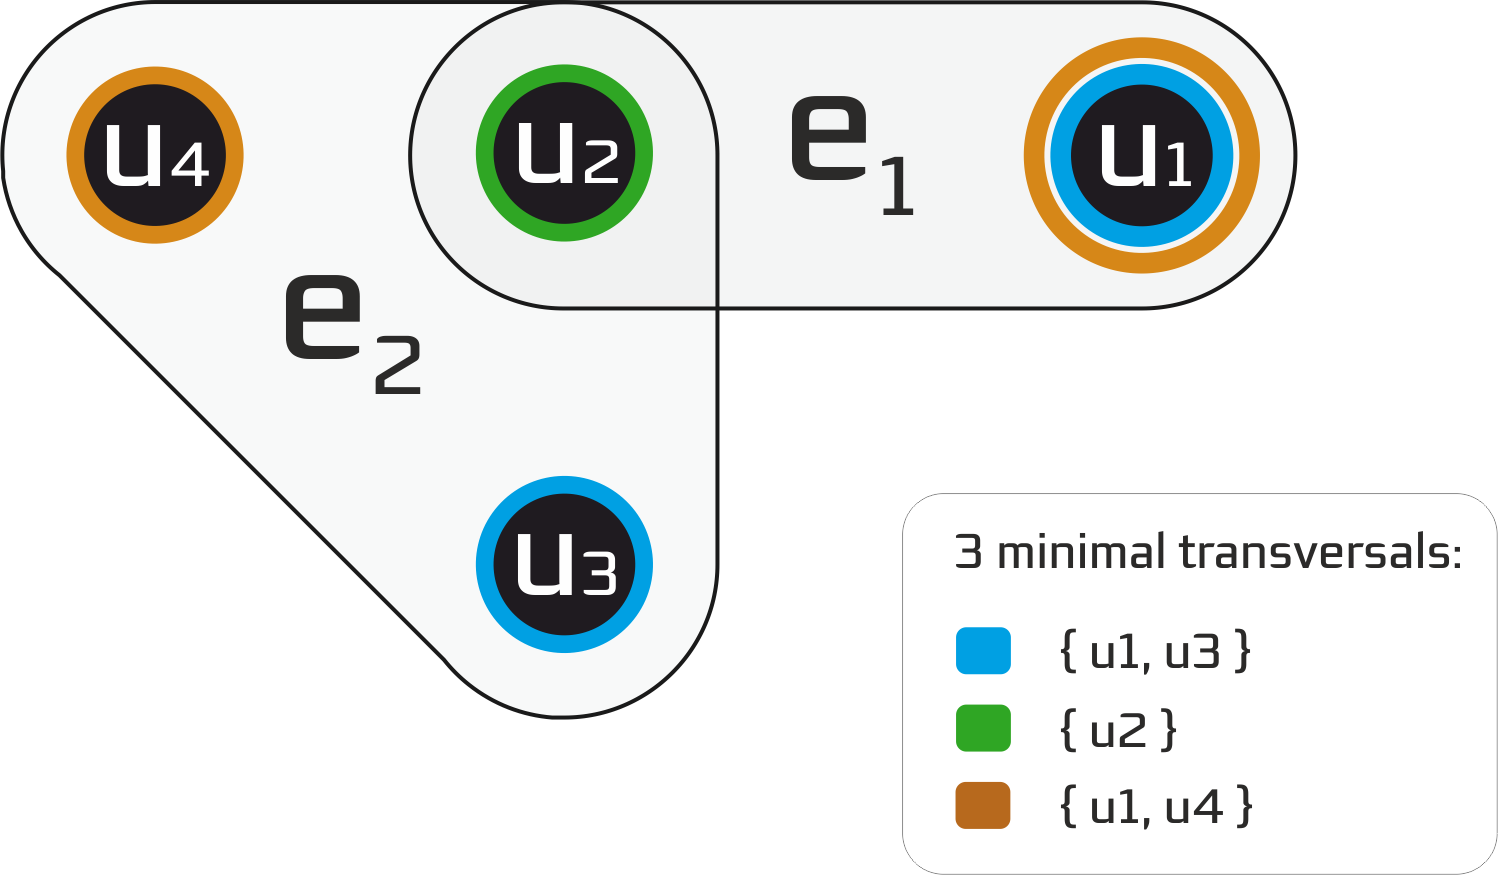
\includegraphics[scale=1]{transversal_example.png}
	\caption{Color-coded Transversals}
	\label{transversalexample}
\end{figure}


Another well-studied hypergraph-related problem is hypergraphs clustering. This is done by regarding the edges as node attributes and using several techniques to cluster nodes with similar attributes together. For instance~\cite{zhou2006learning}, proposes powerful methods of spectral clustering on hypergraphs and algorithms for classification and embedding. The methods proposed had a significant advantage when used in hypergraphs over simple graphs, since they managed to store complex relationships among objects on the hyperedges. A game theoretic approach to hypergraph clustering is found in~\cite{bulo2009game}. Specifically, there the cluster is treated as the game-theoretic concept of equilibrium, and the problem of partitioning the hypergraph to clusters as non-cooperative multiplayer game. This has several advantages over classical approaches, e.g. the final number of clusters is not needed beforehand. Finally, Leordeanu and Sminchisescu~\cite{leordeanu2012efficient} propose an efficient clustering method that updates which vertices correspond to which clusters in parallel through an iterative procedure. This manages to reduce computing requirements significantly.



In addition, there are also many ways for matrices to represent a hypergraph or specific attributes of it. For instance the incidence matrix, weight matrix and adjacency matrix are all easily defined, as we show in Section~\ref{sec:Clustering}.

Hypergraphs thus, are a powerful and well-defined way to store information. For example we can easily store (better explained in Chapter~\ref{Chapter6_approach}) EVs in hyperedges that represent a specific quality. Edges then store both attributes of EVs and, possibly, complex relations between them. This comes with advantages like the instant selection of interesting parts of the graph or fast set operations like {\em intersection} or {\em union}.

Later, in Chapter~\ref{Chapter6_approach} we explain how these advantages and the existing literature is exploited for efficient coalition formation.



%----

%Electric vehicles (EVs) are a promising new concept for the automotive industry. EVs use energy stored in a battery and electric motors to generate propulsion. Electricity offers many advantages %against petrol-powered vehicles. Specifically, EVs are cost effective and require less maintenance, and thus have no emissions since they run in electricity powered engines. The growing popularity of EVs %gives rise to the so-called G2V and V2G problems. G2V describes a system where EVs connect and draw power from the Grid without overloading it\cite{valogianni2014effective}. V2G is the problem of EVs %communicating with the Grid in order to either lower their power demands or return power back to the network when there is a peak in the request for power. This helps the Grid to maintain a balanced power %load\cite{ramchurn2012putting}. This is the problem we will be dealing with in this paper.

%	An important issue in the V2G problem is that there are possibly millions of EVs which communicate and connect to the Grid. The vast number of vehicles means that we must create the most appropriate %groups to cover the needs of the Grid at any given time. Algorithms that scale well and give results almost instantly are necessary. 

%	In order to tackle the V2G problem, we resort to coalition formation. Specifically, we propose the formation of coalitions using hypergraphs. By doing so, we can efficiently locate reliable agents and form %effective EV cooperatives to provide sufficient energy and stability. 

%	Such attempts use mostly machine learning or attempting to form the optimal coalition\cite{deORamos2014}\cite{valogianni2014effective}. This had the drawback that it did not scale to more than a few %hundred agents \cite{kamboj2010exploring} \cite{deORamos2014}. Besides, the approaches that have been used do not deal with multi-criteria optimization. This is important, however because in reality %coalitions have to be formed according to several criteria such as capacity and discharge rate. In our attempt, we will try to form coalitions by selecting vehicles from a huge pool of individual EVs using 
% multiple criteria for our selections. 


%	The Grid should be able to advertise the amount of power it requires by both asking for a required capacity and a maximum discharge rate. What we are trying to do is fulfill the required capacity and %discharge rate with the minimum amount of vehicles and by keeping our coalition reliable. We are not searching for an optimal coalition but rather for one that can be generated quickly and reliably. We do %this by organizing our electric vehicles inside a hypergraph. Current research and solutions on the V2G problem do not scale well. It should be noted that it is also the first attempt to use hypergraphs for %coalition generation. Hypergraphs are well studied, and powerful algorithms do exist for traversing and exploring them. 

%	In a few words, we start with a huge pool of EVs. We know their power capacity, discharge rate and if they are committed to connect to the Grid. We also know their reliability. The Grid advertises the demand of a coalition with a specific capacity and discharge rate. We form a coalition that fulfills the power requirements and has a high reliability while also being small in size. 
%	Now in order to build coalitions for the V2G we need to combine the capabilities of EVs. This naturally gives rise to a multi-criterion selection problem for choosing the members of a coalition. In order to tackle this problem, we propose a novel, principled approach in order to form coalitions that have specific characteristics. For this we employ the use of hypergraphs and research that has been done on them \cite{zhou2006learning} \cite{kavvadias2005efficient}

%	In general the related work\cite{kamboj2010exploring}\cite{kamboj2011deploying}\cite{deORamos2014}\cite{valogianni2014effective} focuses in single-criteria coalition formation and in near-optimal %solutions that require great processing power and scale poorly. 

%  ***** AYTO as to exoume ypopsin gia pi8anes erwthseis ****
%First of all, while multiple criteria can usually be expressed as a single one with the help of a utility function, we find that multi-criteria is a more natural way to express the agent's attributes. As such we do not use directly utility functions.

%	To continue while finding the optimal coalition is useful in most cases it can't work in real world situations where there could be millions of EVs, and the requirements could be updated every few seconds. Therefore, we sacrifice the ability to find the optimal solution so that we can process thousands of EV's in a few seconds.